% if you do not like the headers displaying your name and the thesis title, remove the `header` option
\documentclass[header]{macsthesis} 

% the thesis title
\title{Functional Mastermind}

% your name
\author{Kyle Dick}

% your degree programme
\degree{MEng Software Engineering}

% date of submission (can be set to \today to get the date at the time of processing the document)
\date{\today}

% supervisor's name
\supervisor{Kathrin Stark}

% don't mess with this (not a big deal, but still)
% sets up basic PDF metadata
\makeatletter
\hypersetup{
    pdftitle = {\@title},
    pdfauthor= {\@author}
}
\makeatother


\begin{document}

\begin{titlepage}

\begin{center}
	% Title (and subtitle)
	~\\[1cm]
	{\huge \titleColor \textbf{\docTitle}}\\
	~\\[1.5cm]
	
	% Author(s)
	{\huge \docAuthor}\\[1cm]
	{\Large MEng (MA) Software Engineering}\\[0.3cm]
	{\Large 4th Year Dissertation}\\[1cm]
	{\large \textit{Supervised by} {\Large \docSupervisor}}
	~\\[2cm]
	
	% Organisation
	\begin{figure}[h]
		\begin{center}
		
\includegraphics[]{1_front_matter/hwcoa_bw.jpg}
		\end{center}
	\end{figure}	
	~\\[0cm]
	\begin{large}
		\textsc{Heriot-Watt University}\\
		School of Mathematical and Computer Sciences\\
		Department of Computer Science
	\end{large}
	~\\[1cm]
	
	% Date
	{\Large \docDate}\\
	~\\[1.5cm]
	
	% Copyright
	\begin{minipage}{0.7\textwidth}
	\singlespacing
	\begin{footnotesize}
	The copyright in this dissertation is owned by the author. Any quotation from the dissertation or use of any of the information contained in it must acknowledge it as the source of the quotation or information.
	\end{footnotesize}
	\end{minipage}
	
\end{center}

\end{titlepage}

\frontmatter

% This is the required declaration of authorship.
% You don't need to edit this file.
% All the necessary data will be pulled from the definitions in the main file.

\makeatletter

\begin{center}
  \begin{large}
    \textsc{declaration}
  \end{large}
\end{center}

\noindent I, {\@author}, confirm that this work submitted for assessment is my own and is expressed 
in my own words. Any uses made within it of the works of other authors in any form (e.g., 
ideas, equations, figures, text, tables, programs) are properly acknowledged at any point 
of their use. A list of the references employed is included.
 
\bigskip
 
\noindent Signed: {\@author}

\bigskip

\noindent Date: {\@date}

\makeatother

\newpage


\Chapter*{Abstract}

A short description of the project and the main work to be carried out. 
Probably between one and two hundred words. 


\tableofcontents

\mainmatter

\chapter{Introduction}
\label{cha:intro}

\section{Motivation}
\label{sec:intro_motiv}

Mastermind is a codebreaking game played between two players each with opposing goals. The game was originally a board game which would utilise plastic pegs on a board to represent codes and other elements of the gameplay, a brief description of how the game functions is as follows. The code-maker (CM) is tasked with constructing a hidden-code (HC) within the boundaries of set parameters. These parameters can be defined as a length l which the HC must exactly match in it's number of present symbols and a set of symbols s which is used to construct the HC. In the standard variant of the game the length is four symbols whilst the set consists of six symbols of which repeats can be present within the HC.

The code-breaker (CB) is the role designated to the player that is tasked with discovering the contents and arrangement of the HC. This processs involves the CB attemtping guesses at what they believe the HC should be while refining their guesses based on responses given by the CM as to the accuracy of each guess. These responses utilise two metrics to judge the accuracy of a guess. The first metric in a response are white pegs which symbolise that a symbol in the current guess is present within the HC but has been arranged in an incorrect position. The second metric are black pegs which represent a symbol in the guess which is present within the HC and is also in an identical position in both the guess and the HC.

\section{Aim and Objectives}
\label{sec:intro_aim}

So in this dissertation we aim to address this aspects of Y. In particular we want to achieve the following objectives:
\begin{itemize}
    \item Something;
    \item [*] Another thing with different bullet;
    \item The last thing.
\end{itemize}

\section{Methodology}
\label{sec:intro_method}

Here are briefly the main problems, and what approach we used to tackle them.

\section{Contributions}
\label{sec:intro_contrib}

In order, what this dissertation contributes:
\begin{enumerate}
    \item First item.
    \item Second item.
    \item Third item.
\end{enumerate}

\section{Organisation}
\label{sec:intro_orga}

Here is how this dissertation is organised. After motivating and introducing our work (this chapter), we investigate the literature to present the state-of-the-art in \cref{cha:back}. We then present our great solution in \cref{cha:dev}, before evaluating it in \cref{cha:eval}. Finally we conclude in \cref{cha:concl}, highlighting limitations, and possible future work.

\Chapter{Background}

\rule{\textwidth}{2pt}

% Summary of the background material and introduction to the section
The Mastermind puzzle has been subject to investigations regarding solutions to the code-breaking aspect of the game
since its release.
This section will provide background material which aims to give context to the aims and objectives of this project.
The project was inspired by a paper exploring sudoku solutions from a series of problems known as functional pearls,
The processes used to derive those solutions will be used to guide this project in this current stage.
Following this brief introduction is an explanation of the game Mastermind which the solution will be derived from along
with references to previous work by others. The previous work examined will focus on the specific area of search spaces
in regards to finding the optimal best move at each position in the puzzle. At the conclusion of this section the goal is
that the reader has an understanding of the important concepts relating to this project such that the aims and objectives
are clear in their feasibility and relevancy.

\subsection {The Mastermind Puzzle}

The Mastermind puzzle began as a two-player game in which one player seeks to break the code created by the other player \cite{Wolfram}.Originally a physical board game designed by an Isreali Postmaster named Mordecai Meirowitz, distributed through Invicta Toys and Games \cite{Invicta}, the game has evolved into a rich area of investigation due to the strategies
associated with solving its simple rule set.

\subsubsection {The Rules of Mastermind}

% Explanation of Mastermind puzzle
The standard variant of the game as it was introduced in 1970 used a simple plastic board with coloured pegs to represent individual elements for the code.
Each game would begin with a secret code being constructed from c colours and l length, in the standard variant this would result in a code of length four constructed from a set
of six coloured pegs \cite{Wolfram}.

\begin{figure}[H]
\centering
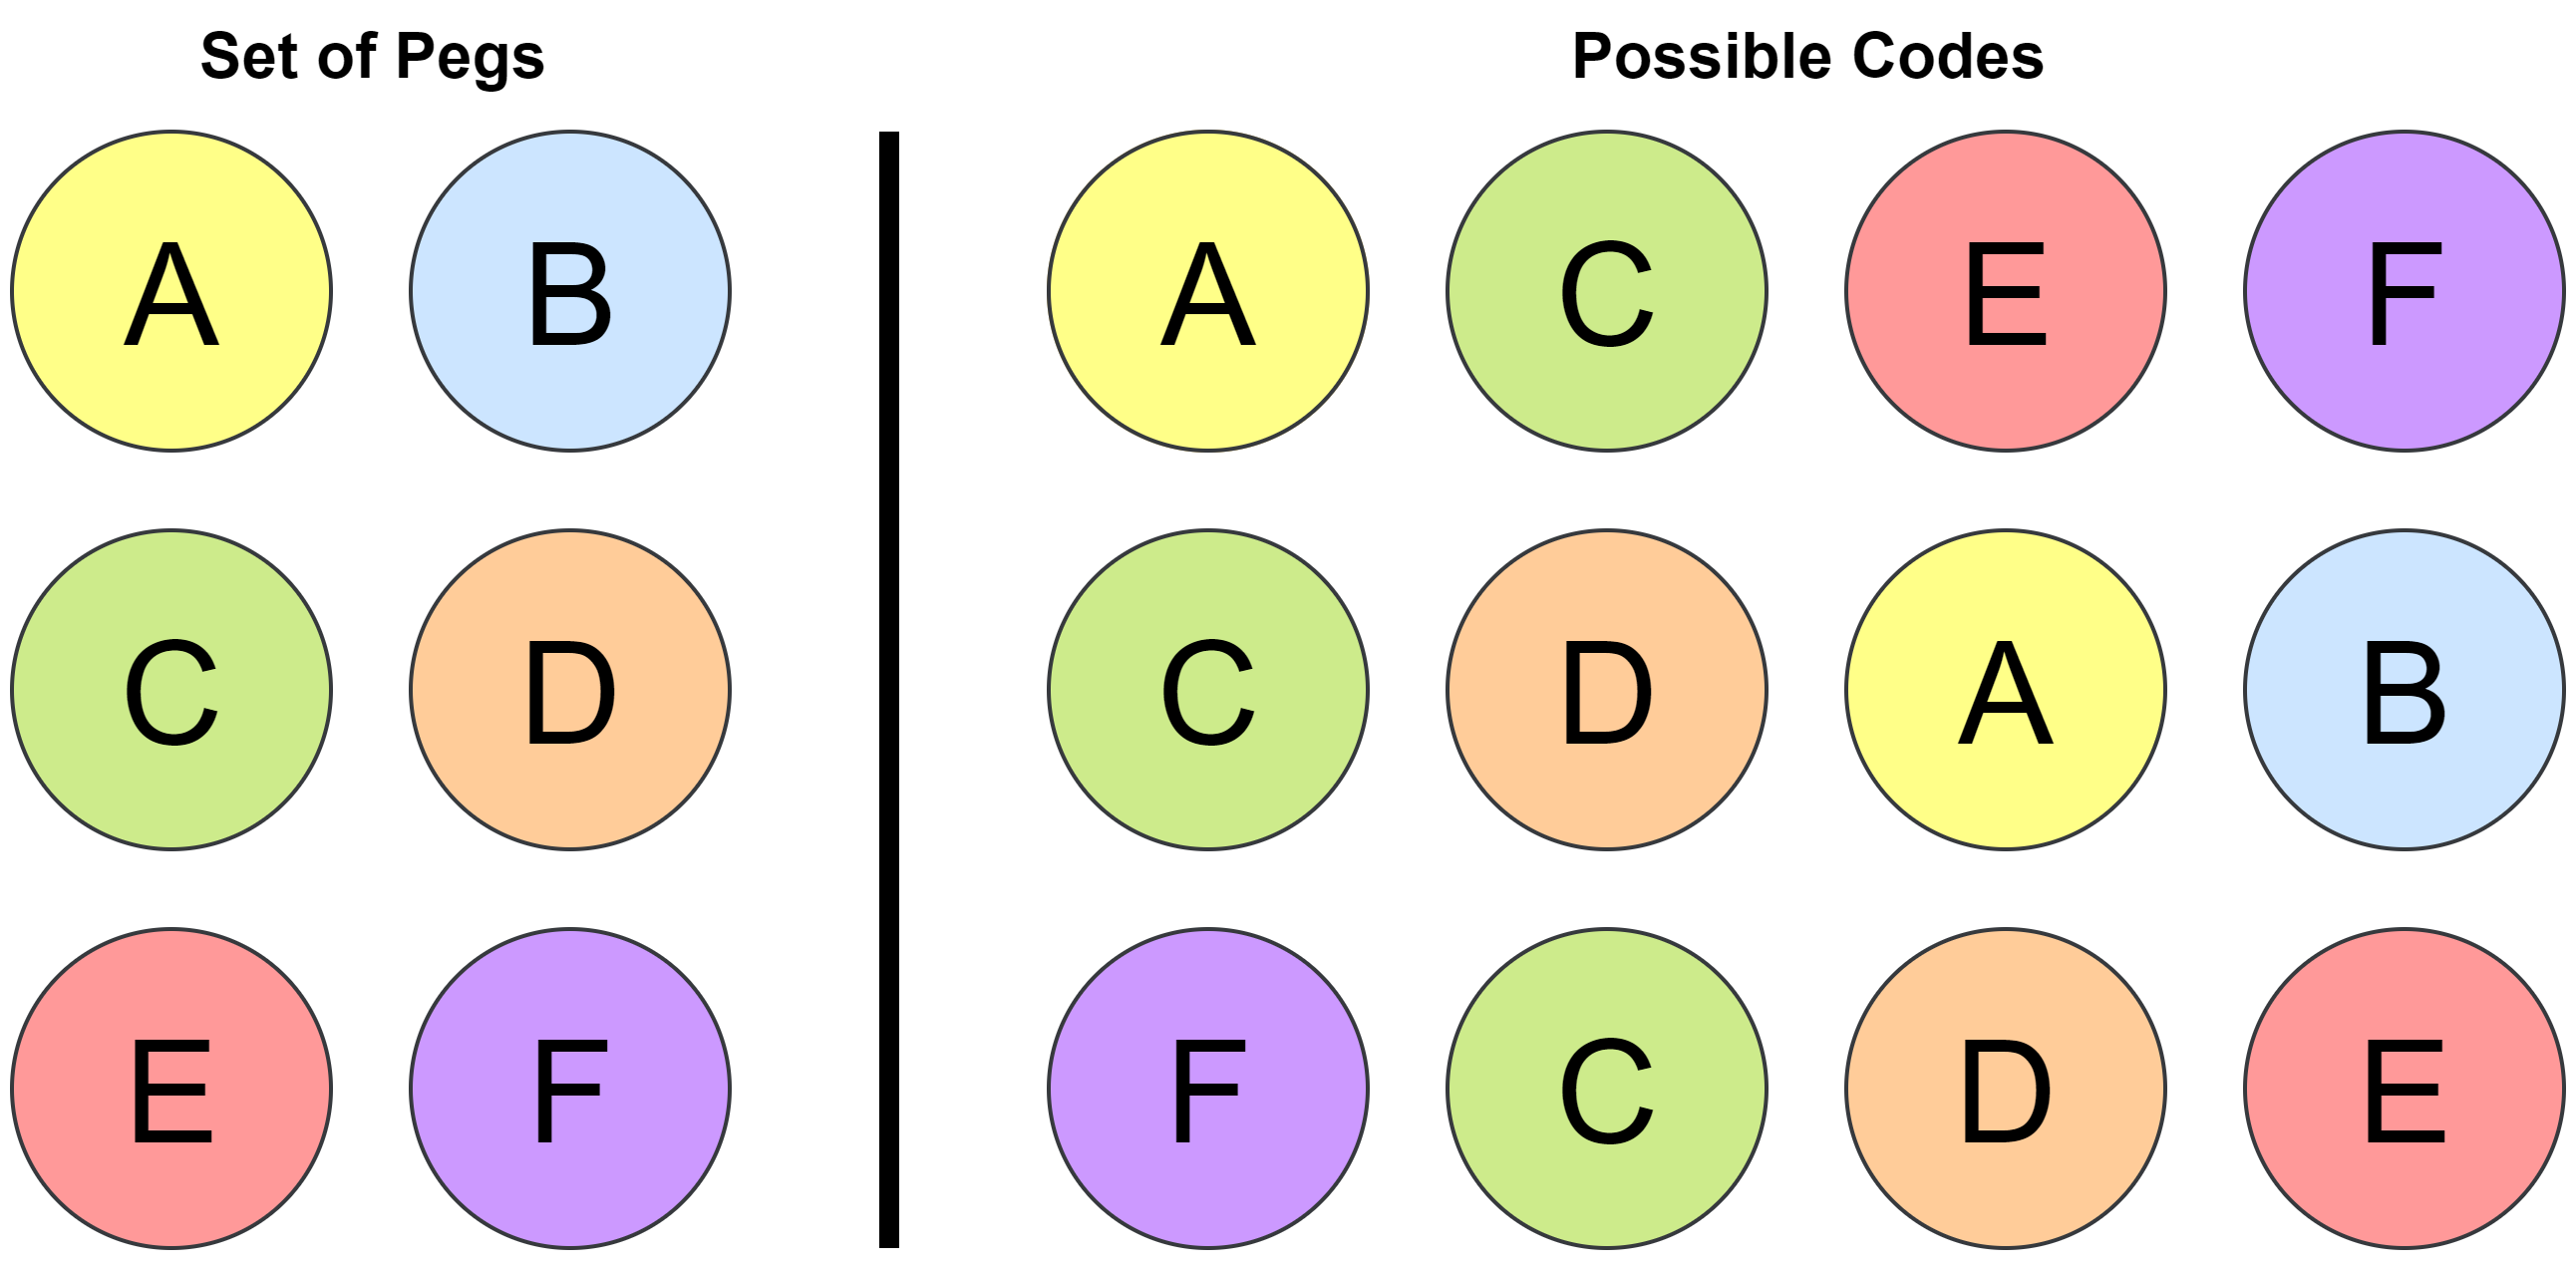
\includegraphics[scale=0.5]{pegs}
\caption{ Example codes which would satisfy the constraints of the standard variant of Mastermind.}
\end{figure}

The codebreaker would attempt several guesses by constructing codes of a similar shape and rewarded with clues as to how closely their guess resembled the hidden code.
The physical game represented these hints as smaller plastic pegs of two colours, one which would denote that a correct colour had been selected but was used in an incorrect
position and one which would confirm that a correct colour and position had been selected for an element.
\begin{figure}[H]
\centering
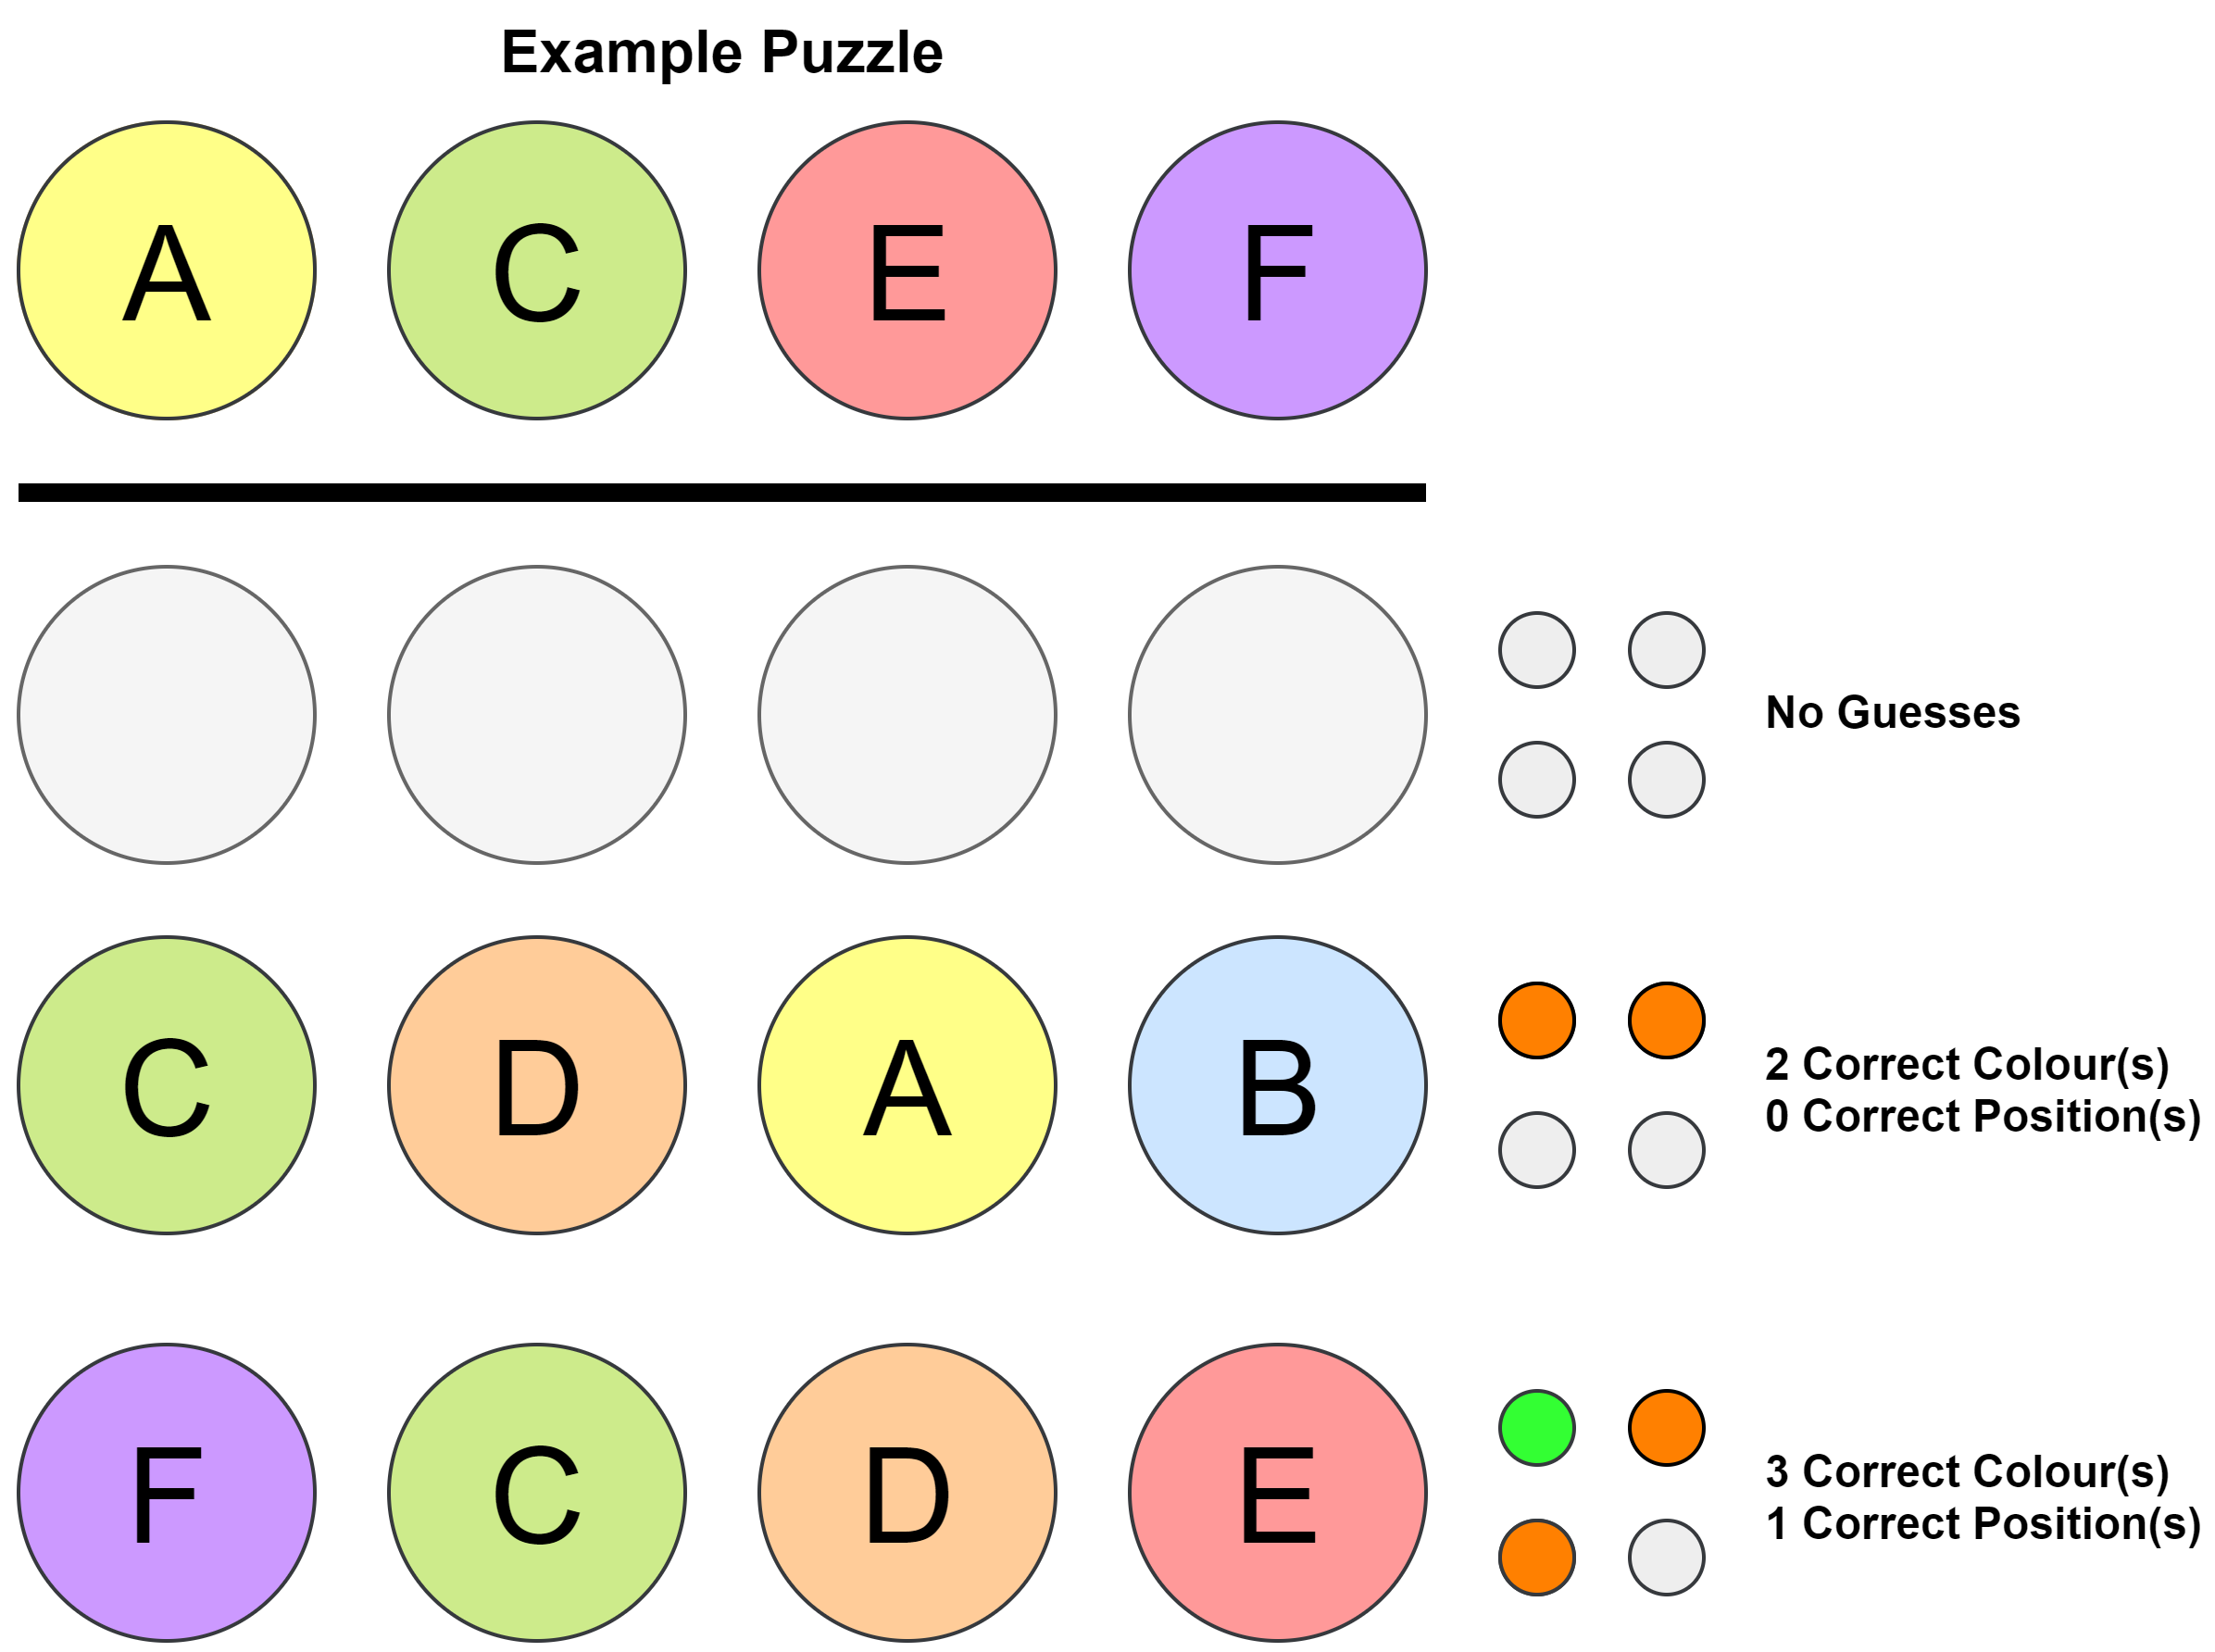
\includegraphics[scale=0.5]{guesses}
\caption{A simplified representation of $CB$ attempting to break the code set by $CM$}
\end{figure}

There are two end states of the game, one in which the code is broken and discovered by the guessing player and one in which the guessing player is unable to discover the code
within a limit of guesses.


\Chapter{Requirements Analysis $\lor$ Research Methodology}

One of the following sections depending on the style of the project:  
\begin{itemize}
\item \textbf{Requirements  Analysis:}  This  is  required  for  technical  projects  and  should  be 
                                        linked back to the project aim and objectives. It should provide a detailed use case 
                                        scenario  and  suitable  use  case  descriptions,  user  requirements,  and  MoSCoW 
                                        analysis of the requirements.  
\item \textbf{Research  Methodology:} This  is  required  for  research  projects  and  should  be 
                                      linked  back  to  the  project  aim  and  objectives.  It  should  describe  the  research 
                                      methods that will be employed in the project and the research questions that will 
                                      be investigated.
\end{itemize}

\rule{\textwidth}{2pt}

\lipsum


\Chapter{Design}

An initial design of software or sketch of the research methodology, assuming there is something to report.
This part is optional, but good to include if there is something substantial to say.

\rule{\textwidth}{2pt}

\lipsum


\Chapter{Evaluation Strategy}

Details of the evaluation and analysis to be conducted.

\rule{\textwidth}{2pt}

\lipsum


\Chapter{Project Management}

This section should include: 
\begin{itemize}
\item A timetable  for  the  whole year  agreed  with  your supervisor  and  specifying activities, deliverables and deadlines. 
\item An analysis of the risks for the project together with appropriate mitigation plans, i.e. not due to illness. 
\item A well-researched  consideration  of  any  professional,  legal,  ethical,  and  social issues  pertinent  to  the  project. 
     (E.g., codes  of  conduct  (BCS),  codes  of  practice, standards,  computer law,  ethical  decision  making,  social aspects, copyright, tradematks, patents, data protection, etc.)
\end{itemize}

\rule{\textwidth}{2pt}

\lipsum


\bibliographystyle{abbrvnat}
\bibliography{bibliography}

\appendix

\Chapter{Examples of using \LaTeX}

\Section{Citations}

Two main ways to cite are:
\begin{itemize}
  \item \textbf{parenthetical:} The importance of computable real numbers \citep{Turing-computable-numbers} in this work~[\dots]
  \item \textbf{in-text:} We will follow the notation style used by \citet{Sipser-textbook}.
\end{itemize}



\end{document}
